\section{Supplementary Material}

\begin{figure}[h]
    \centering
    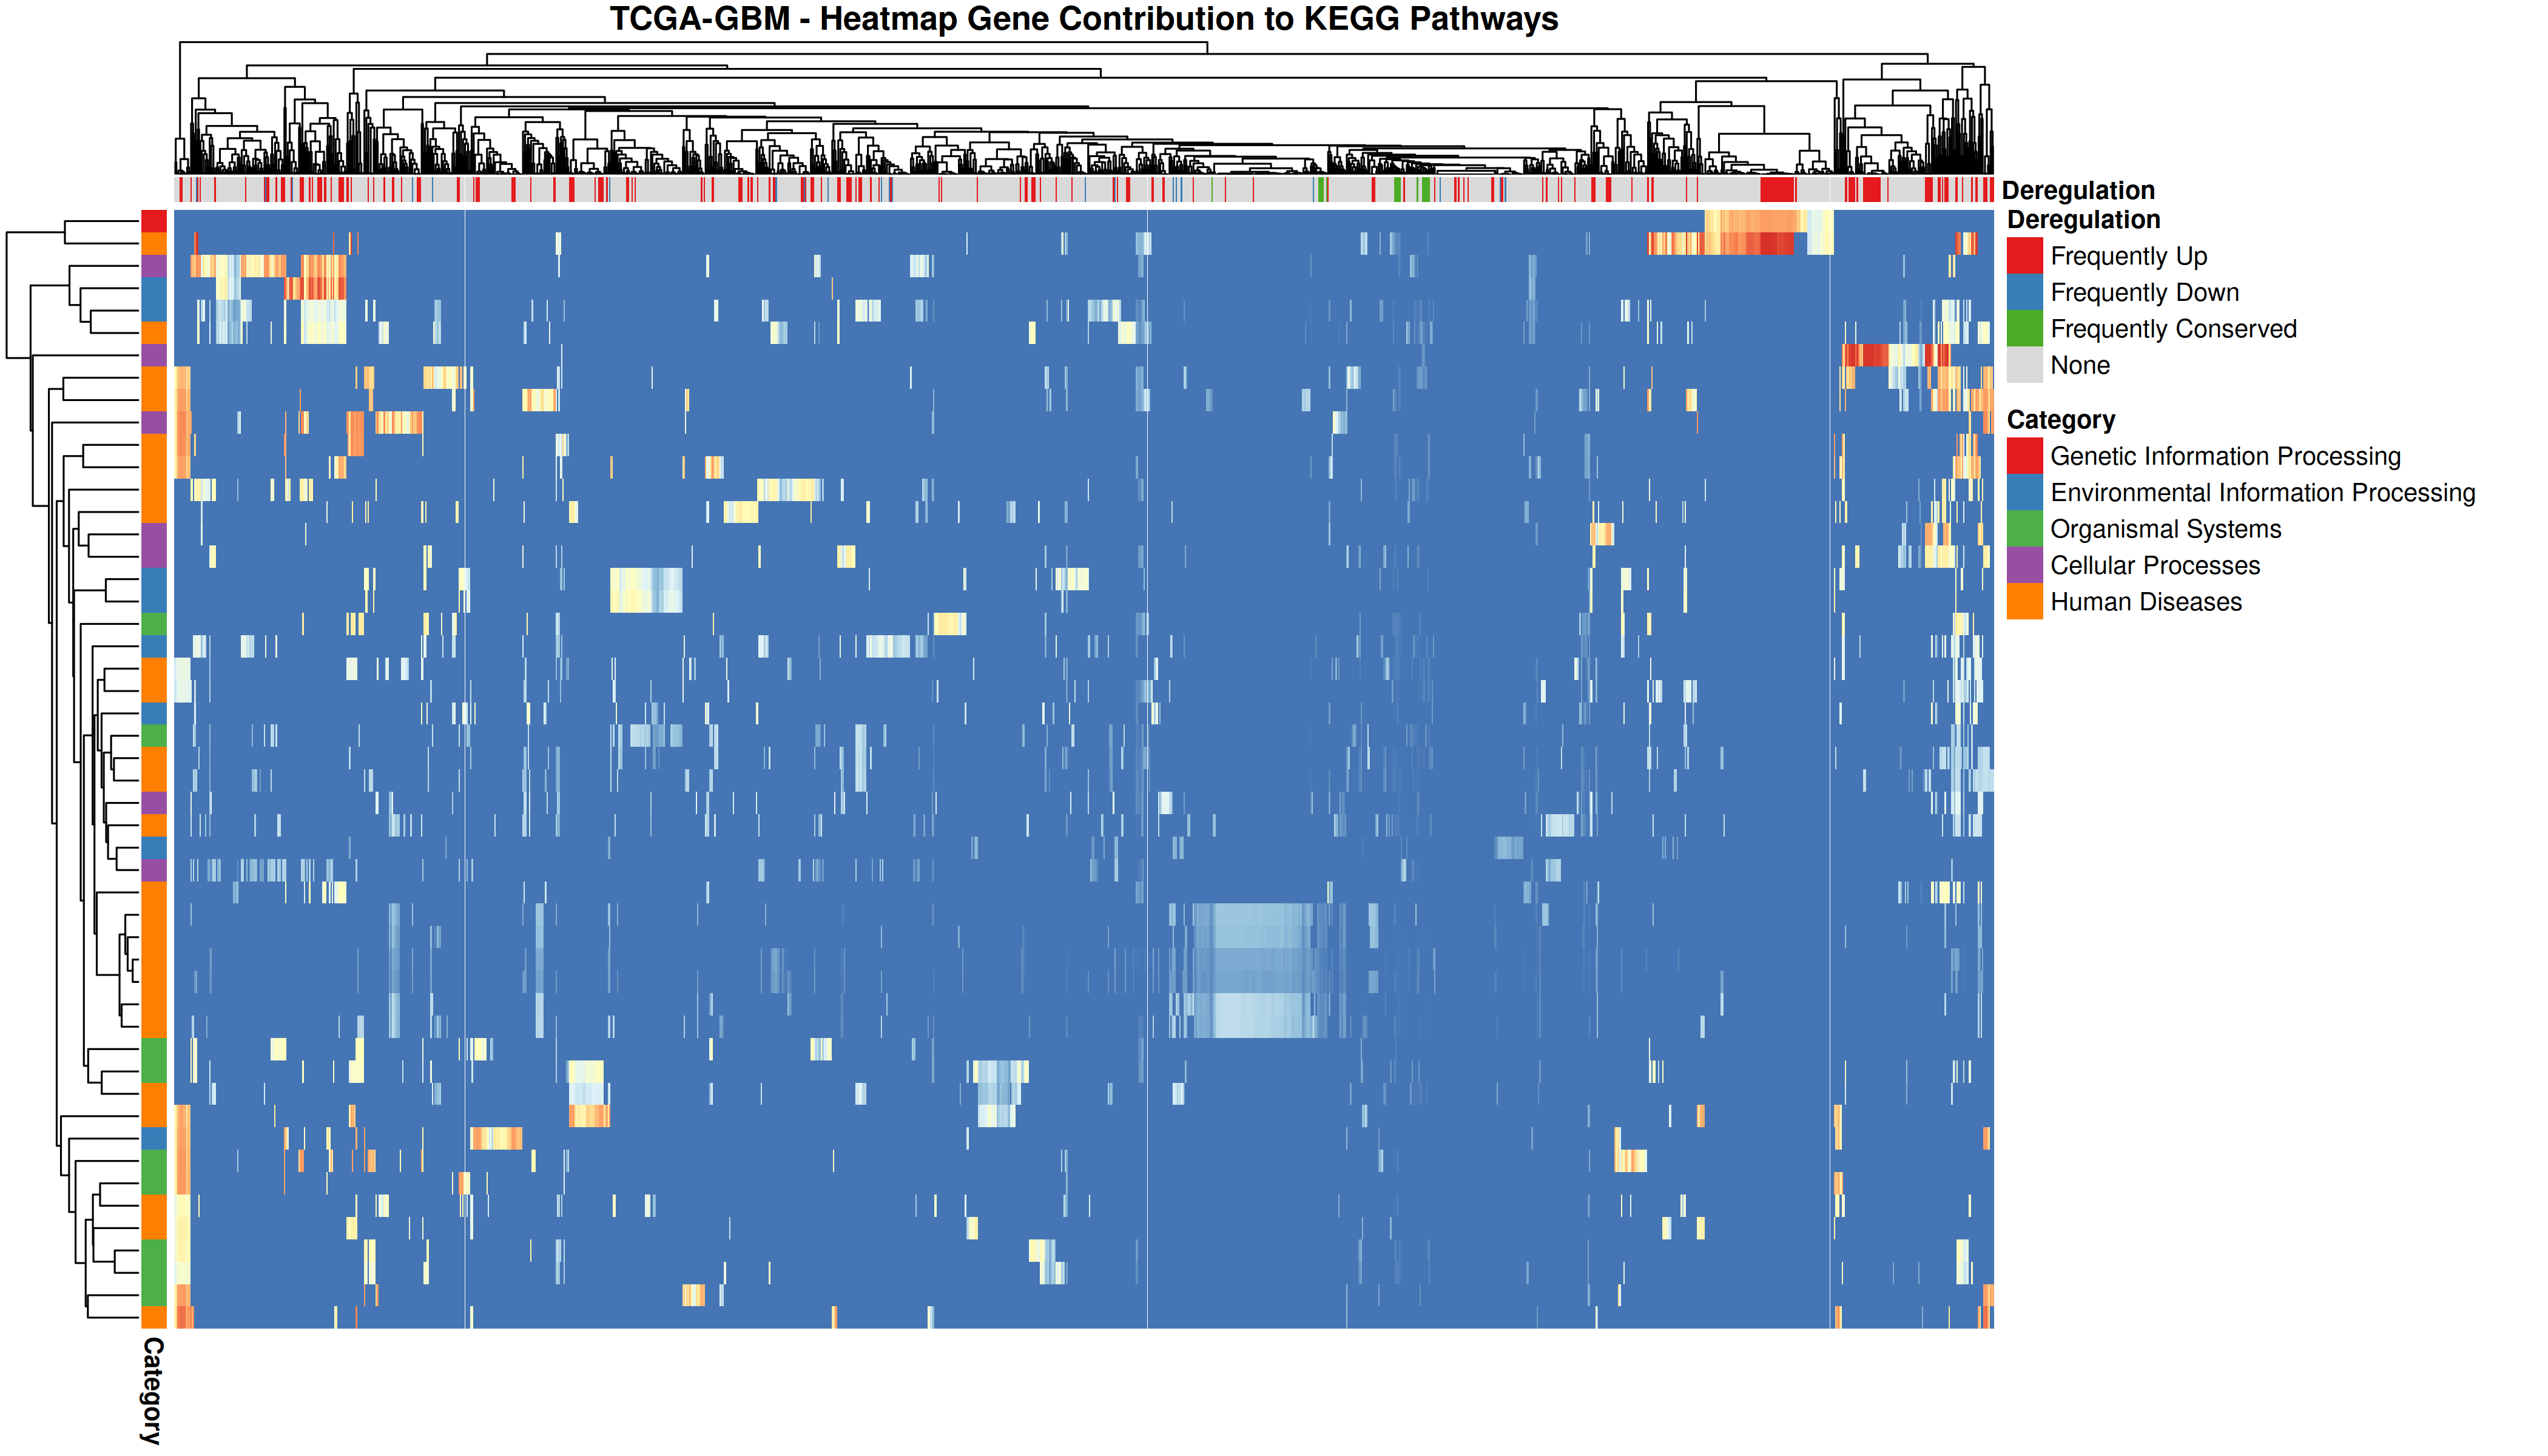
\includegraphics[width=\textwidth]{img/gene_contrib_kegg_tcga}
    \caption {
        Heatmap of the gene contributions for each pathways with \acrshort{tcga} data and \acrshort{kegg} categories.
        Genes contribution to a pathway is computed by calculating how many times a gene appear in the enrichment result for a pathway.
        Red colour indicates a strong contribution and blue colour indicates a week contribution.
        Only genes with a total contributions higher than the third quartile and pathways where the total gene contribution is higher than the third quartile are kept.
        Pathways are colored by their categories.
        Genes are colored by their deregulation frequency : red indicates genes that are up-regulated in 90\% of the samples, blue indicates genes that are down-regulated in 90\% of the samples, green indicates genes that are not deregulated in 90\% of the samples and grey genes that correspond to none of the above.
    }
    \label{supp:gene-contrib-kegg-tcga}

\end{figure}

\begin{figure}[h]
    \centering
    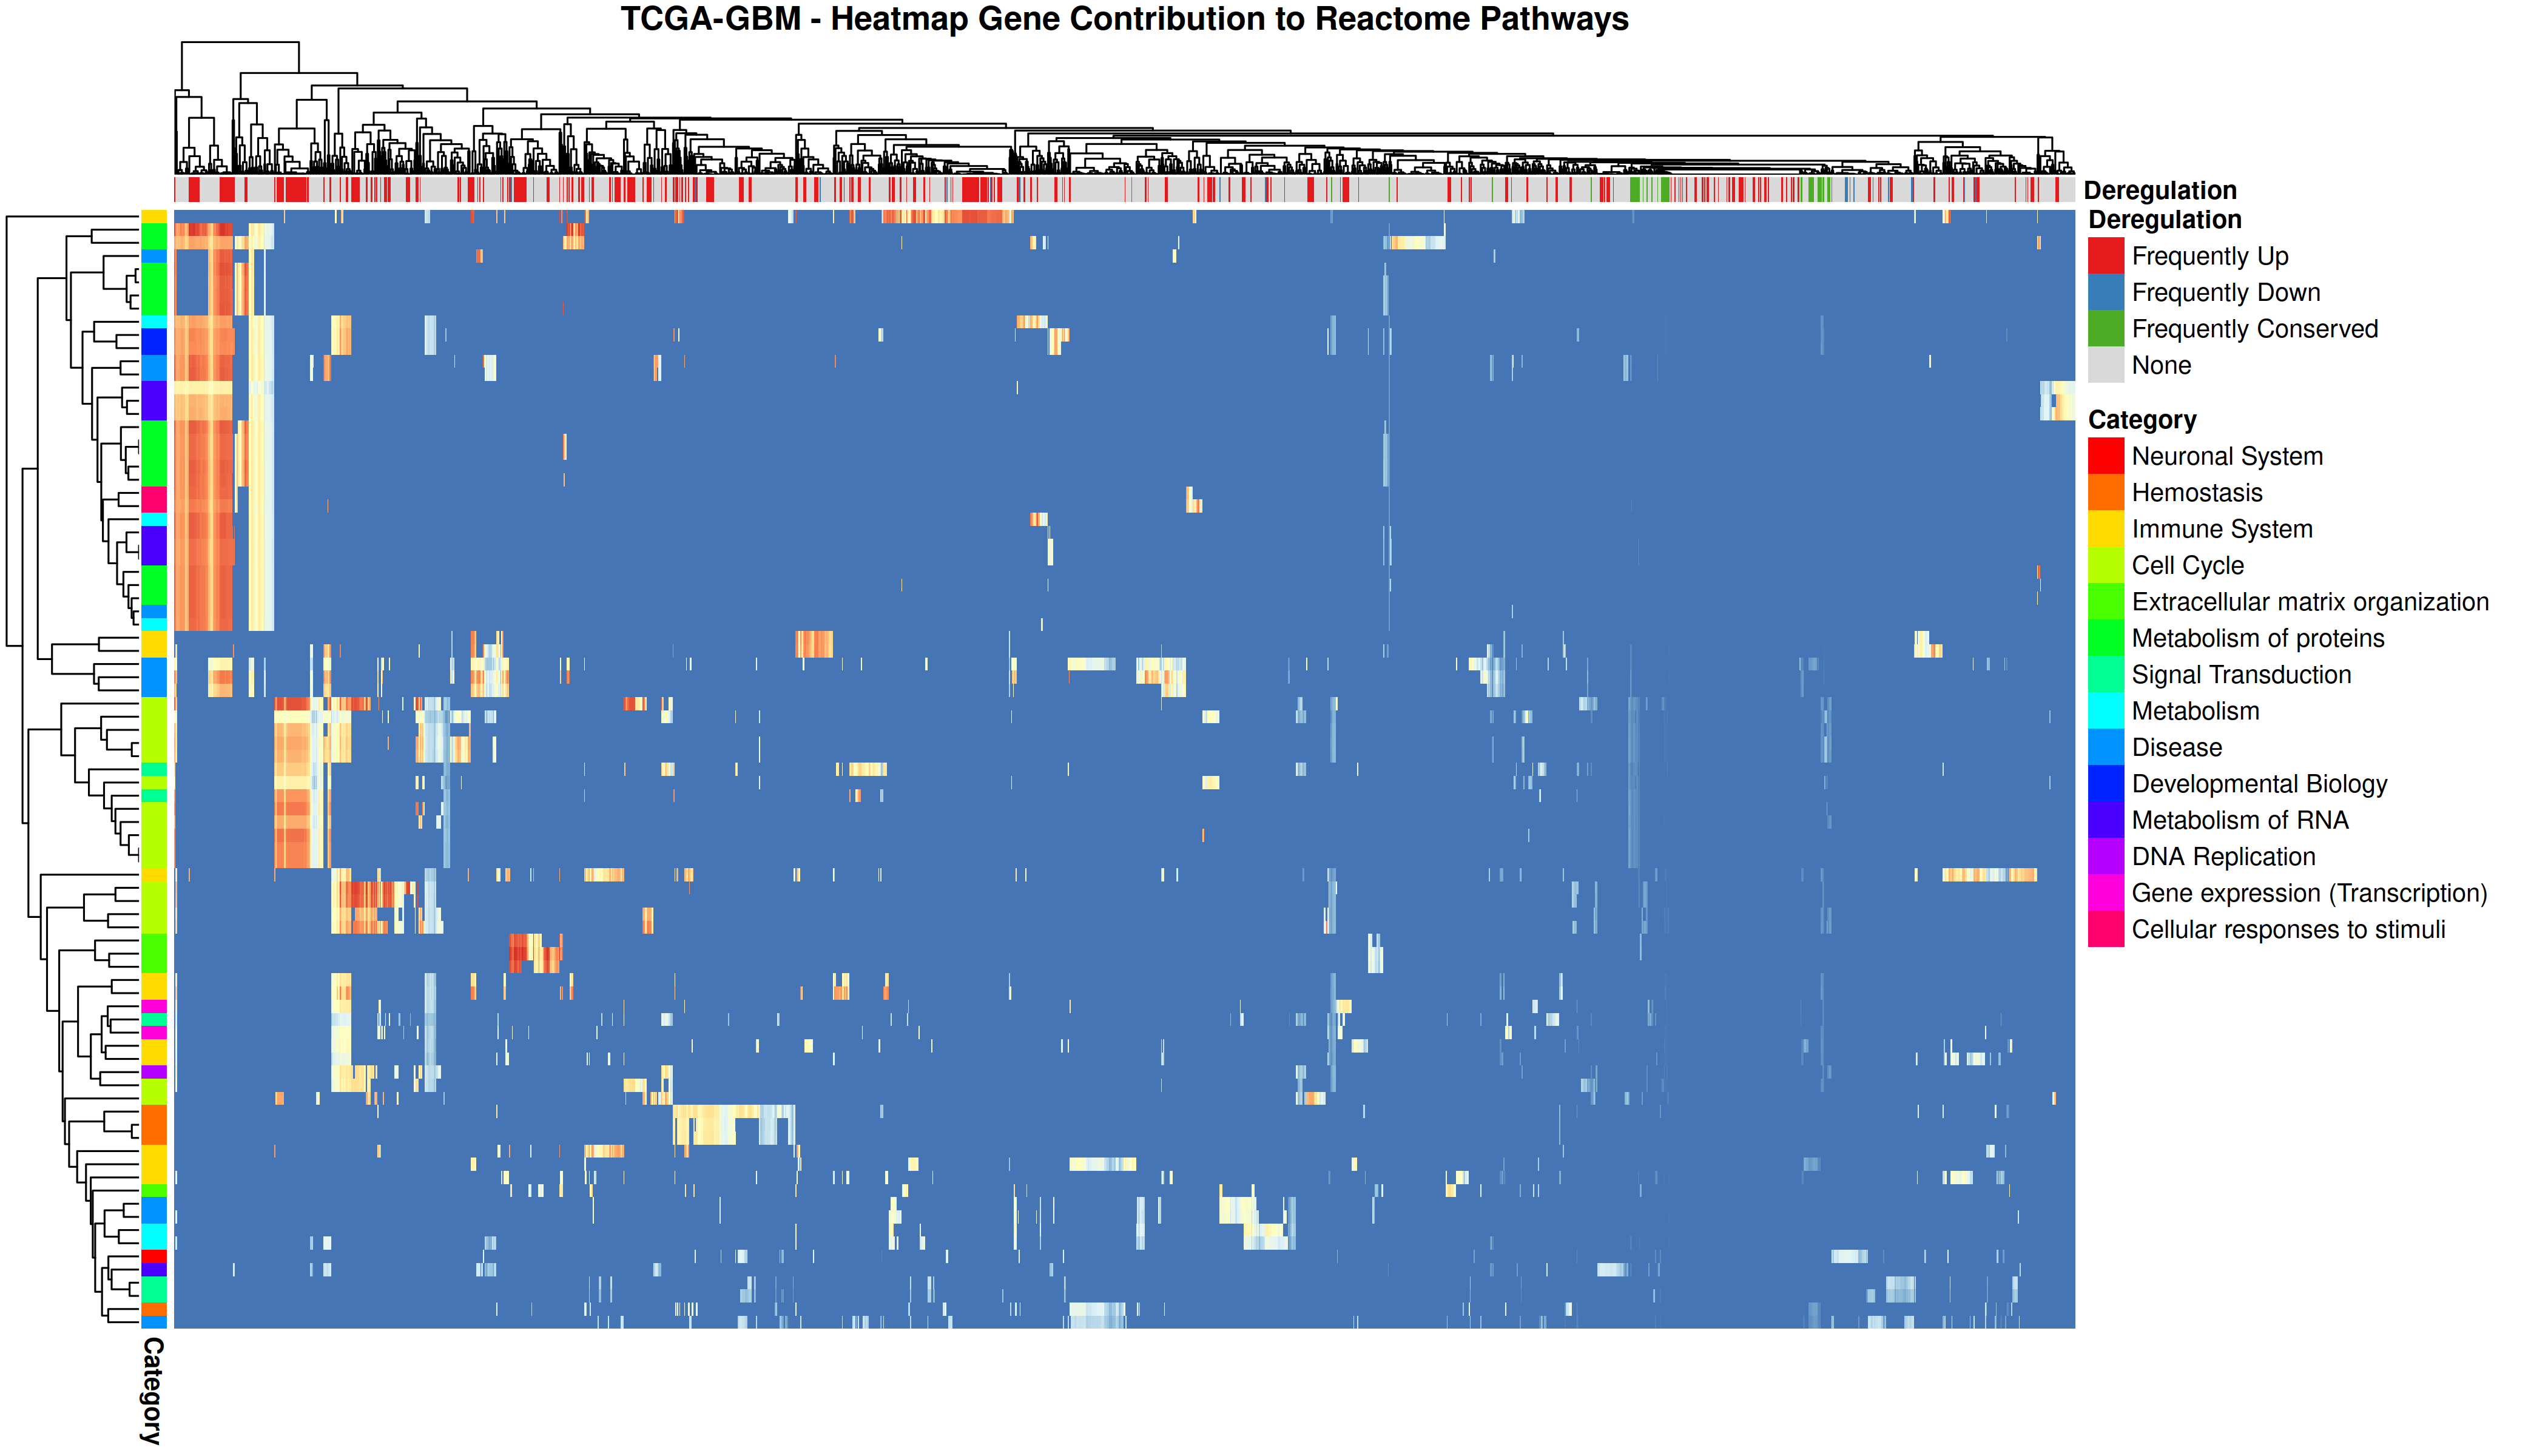
\includegraphics[width=\textwidth]{img/gene_contrib_reactome_tcga}
    \caption {
        Heatmap of the gene contributions for each pathways with \acrshort{tcga} data and Reactome categories.
        Genes contribution to a pathway is computed by calculating how many times a gene appear in the enrichment result for a pathway.
        Red colour indicates a strong contribution and blue colour indicates a week contribution.
        Only genes with a total contributions higher than the 90\% percentile and pathways where the total gene contribution is higher than the third quartile are kept.
        Pathways are colored by their categories.
        Genes are colored by their deregulation frequency : red indicates genes that are up-regulated in 90\% of the samples, blue indicates genes that are down-regulated in 90\% of the samples, green indicates genes that are not deregulated in 90\% of the samples and grey genes that correspond to none of the above.
    }
    \label{supp:gene-contrib-reactome-tcga}
\end{figure}